\documentclass[a4paper, 11pt]{article}

\usepackage{helvet}
\usepackage{graphicx}
\usepackage[hyphens]{url}
\usepackage{hyperref}
\usepackage[all]{hypcap} 
\usepackage{xcolor}
\usepackage{listings}
\usepackage[T1]{fontenc}
\usepackage{verbatim}
\usepackage{mathtools}
\usepackage{float}
\usepackage{csquotes}

\usepackage{comment} % enables the use of multi-line comments (\ifx \fi) 

\usepackage{fullpage} % changes the margin
\usepackage{longtable}
\usepackage{graphicx}
\usepackage{fancyvrb,xcolor}
\usepackage{listings}
\usepackage{color}
\usepackage[margin=3cm]{geometry}
\usepackage{relsize}
\definecolor{dkgreen}{rgb}{0,0.6,0}
\definecolor{gray}{rgb}{0.5,0.5,0.5}
\definecolor{mauve}{rgb}{0.58,0,0.82}
\definecolor{LightCyan}{rgb}{0.88,1,1}
\usepackage{float}
\usepackage{caption}
\DeclareCaptionFont{white}{\color{white}}
\DeclareCaptionFormat{listing}{\colorbox{gray}{\parbox{\textwidth}{#1#2#3}}}
\captionsetup[lstlisting]{format=listing,labelfont=white,textfont=white}
\newcommand{\bigqm}[1][1]{\text{\larger[#1]{\textbf{?}}}}
\lstset{
  language=Java,
  aboveskip=3mm,
  belowskip=3mm,
  showstringspaces=false,
  columns=flexible,
  basicstyle={\small\ttfamily},
  numbers=none,
  numberstyle=\tiny\color{gray},
  keywordstyle=\color{blue},
  commentstyle=\color{dkgreen},
  stringstyle=\color{mauve},
  breaklines=true,
  breakatwhitespace=true,
  tabsize=3
}
\graphicspath{ {images/} }

\lstset{
    basicstyle=\scriptsize,
    numbers=left,
    numberstyle=\scriptsize,
    stepnumber=1,
    numbersep=5pt,
    showspaces=false,
    showstringspaces=false,
    showtabs=false,
    frame=shadowbox,
    tabsize=4,
    captionpos=b,
    breaklines=true,
    breakatwhitespace=false,
    keywordstyle=\color{blue!70},
    commentstyle=\color{red!50!green!50!blue!50},
    rulesepcolor=\color{red!20!green!20!blue!20},
    numberbychapter=false,
    stringstyle=\ttfamily
}

\setcounter{tocdepth}{2}

\hypersetup{
    colorlinks=true,
    breaklinks=true,
    urlcolor=blue,
    linkcolor=black
}

\begin{document}

\author{Hussam Hallak\\
CS Master's Student}
\title{Old Dominion University\\
Department of Computer Science\\
CS834: Introduction to Information Retrieval\\
Fall 2017\\ 
Assignment 5\\
Professor: Dr. Michael Nelson}
\maketitle
\newpage

%\tableofcontents
%\listoffigures
%\listoftables

\section*{Question 1:}
Exercise 6.2: 

Create a simple spelling corrector based on the noisy channel model. Use a single-word language model, and an error model where all errors with the same edit distance have the same probability. Only consider edit distances of 1 or 2. Implement your own edit distance calculator (example code can easily be found on the Web).

\subsection*{Answer:}
I have used the WikiSmall collection provided on the book website as a sample:

http://www.search-engines-book.com/collections/



\pagebreak
Google found about 377,000,000 results for the term ``Memory''.
\begin{figure}[h]
\caption{Query: Memory, Search Engine: Google}
\centering
%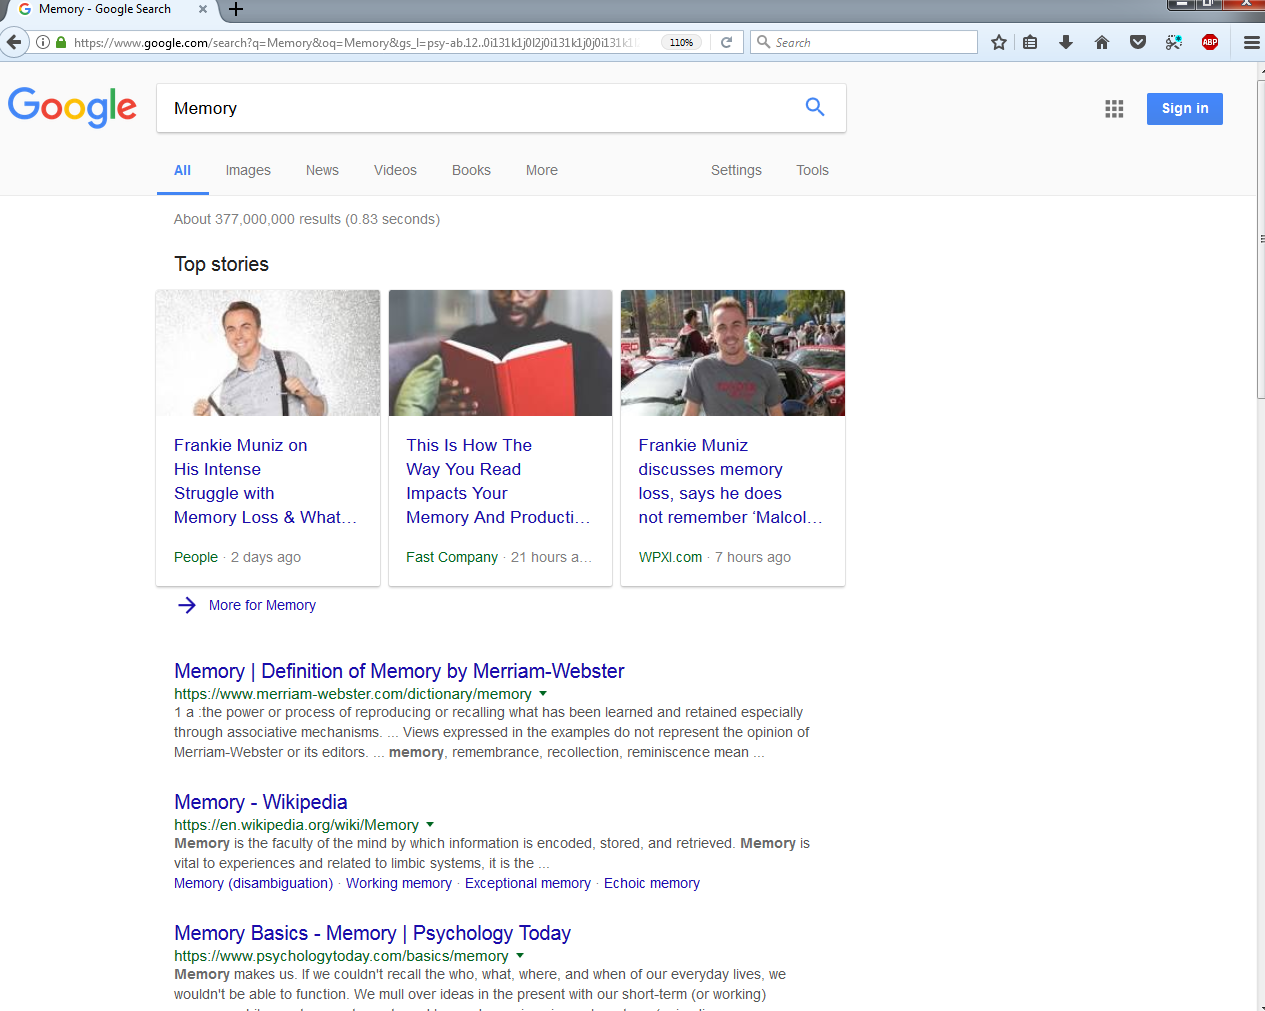
\includegraphics[scale=0.4]{Q1/MemoryGoogle.png}
\end{figure}

\section*{Question 2:}
Exercise 10.5: 

Find a community-based question answering site on the Web and ask two questions, one that is low-quality and one that is high-quality. Describe the answer quality of each question.

\subsection*{Answer:}

I chose to use Yahoo! Answers and asked the following question as a high quality one:


Will Turkey leave NATO and form a coalition with Russia and Iran after US backed Syrian Kurds and moved US embassy in Tel Aviv to Jerusalem?

I consider this as a high quality question because of its correct grammar and punctuation. It also targets the kind of users that care about politics who are normally serious people. The question is about the possibility of a certain outcome as a result of current events. The answer should be definitive, either yes or no.

Below is a screen shot of the answers I got:


\begin{figure}[h]
\caption{Answers for high quality question}
\centering
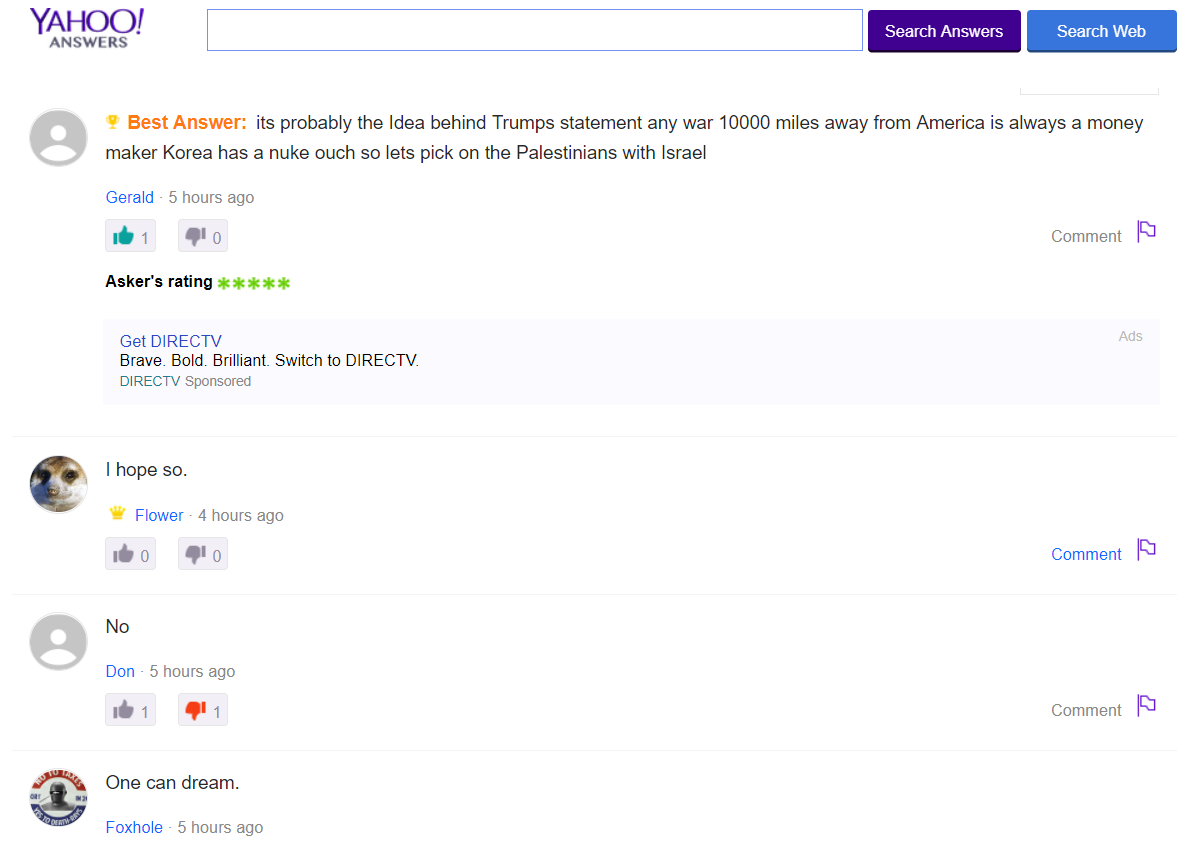
\includegraphics[scale=0.6]{Q2/high.png}
\end{figure}


I marked the answer that has a short analysis of why Turkey might leave NATO as best answer. The answers are high quality and meant to answer the question, but they are short, which is expected.  

I asked the following question as a low quality one: 

Why did you Trump to helb tha kill Saudi to Yemen? Are you forget wat hapend at 11 septemper? Saudi mans kil 3000 America at airplain atak.?

I discovered that asking a low quality question is not an easy task. I was finally able to do it by writing a question then injecting/removing pronouns, verbs, and preposition to produce wrong grammar. I also misspelled some words to make it worse. 

Below is a screen shot of the answers I got:


\begin{figure}[h]
\caption{Answers for low quality question}
\centering
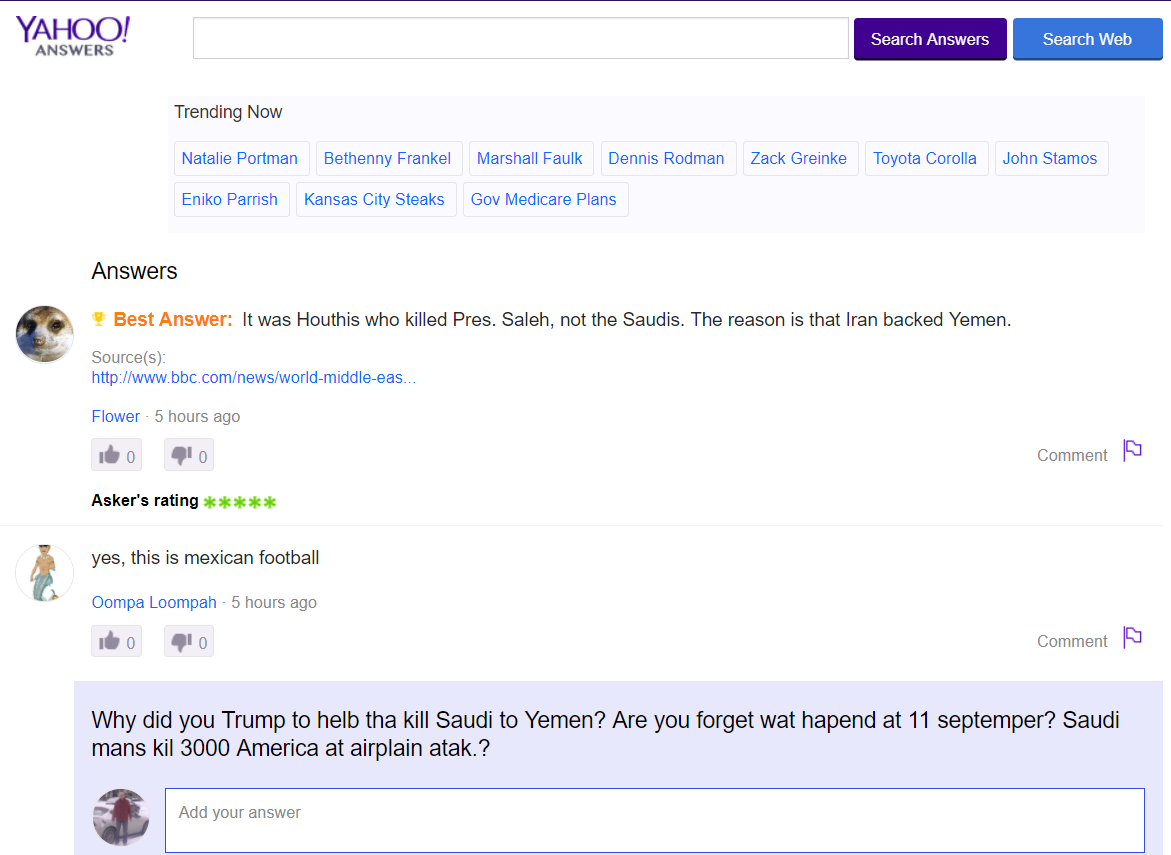
\includegraphics[scale=0.6]{Q2/low.png}
\end{figure}


Surprisingly, I got an answer that is, to a certain extent, related to the topic of the question. I would call that a high quality answer because I do not think that it is possible to come up with a much better answer. The answer includes a source link from BBC. 

For the other answer, I thought that was funny, but it turns out that Yahoo! put my question in the Mexican football category within sports, and that explains why I got this answer. It is, of course, a low quality answer, and it is definitely not related to the question.

\textbf{Observation:}

The results were as expected; low quality questions get low quality answers, and high quality questions get high quality answers.

\section*{Question 3:}
Exercise 10.6: 

Find two examples of document filtering systems on the Web. How do they build a profile for your information need? Is the system static or adaptive?


\subsection*{Answer:}

For my two examples I have chosen Amazon and Youtube. Both of them use an adaptive system for making recommendations. 

Amazon is an e-commerce company. I use it sometimes to purchase different items including car parts, electronics, and other items. The screen shot below shows recommended items for me based on items that I viewed, fuel pumps, and items I purchased recently, a cable to connect my truck to my laptop and perform different diagnosis and scanning. Other recommended items are products that were viewed or bought by people whose purchase history is similar to mine. Amazon does such a good job as far as recommendations. I would buy all the recommended items if I had enough money to splurge. 

\begin{figure}[h]
\caption{Recommended items by Amazon}
\centering
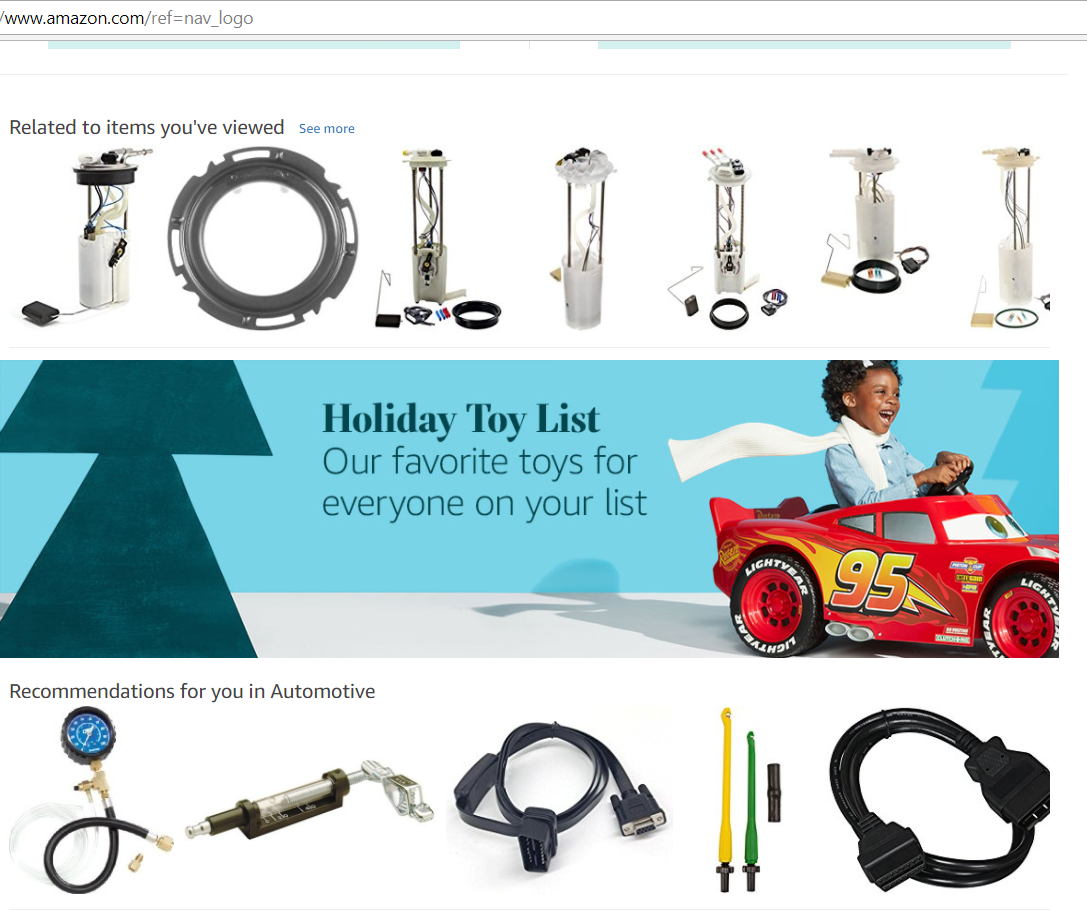
\includegraphics[scale=0.6]{Q3/amazon.png}
\end{figure}

\pagebreak

Youtube is my favorite website. The reason is that I use it for everything including entertainment, news, music, nutrition, and fitness videos. I also watch short lectures or tutorials about concepts I do not understand in Computer Science. Youtube recommends videos for me based on other videos I watched. It also recommends channels/users for me to subscribe to based on videos I watched or other channels I am subscribed to. It also shows popular uploads from channels I am subscribed to.

The screen shot below shows a list of recommended videos, based on videos I watched recently. The recommended videos belong to different categories including entertainment, news, music, fitness, boxing, UFC, ...etc.

\begin{figure}[h]
\caption{Recommended items by Youtube}
\centering
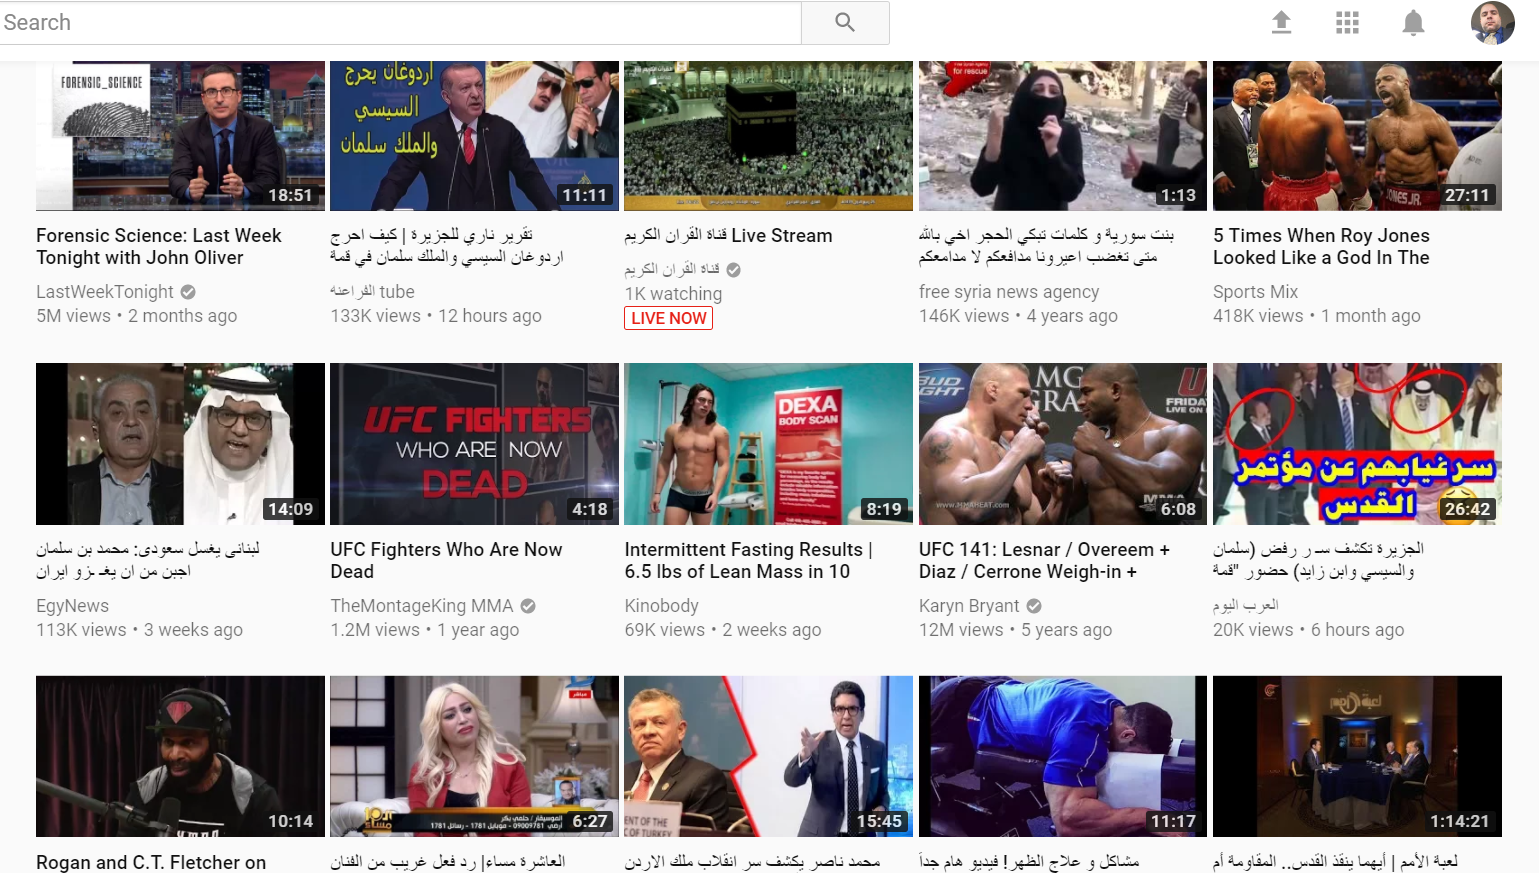
\includegraphics[scale=0.45]{Q3/yrv.png}
\end{figure}

\pagebreak

The screen shot below shows a list of popular uploads from a nutrition channel I am subscribed to, Dr. Josh Axe, as well as a recommended channel for my to subscribe to based on videos I watched and channels I am subscribed to. The recommended channel is an Arabic media channel that posts news from the middle east and other videos about politics.

\begin{figure}[h]
\caption{Recommended items by Youtube}
\centering
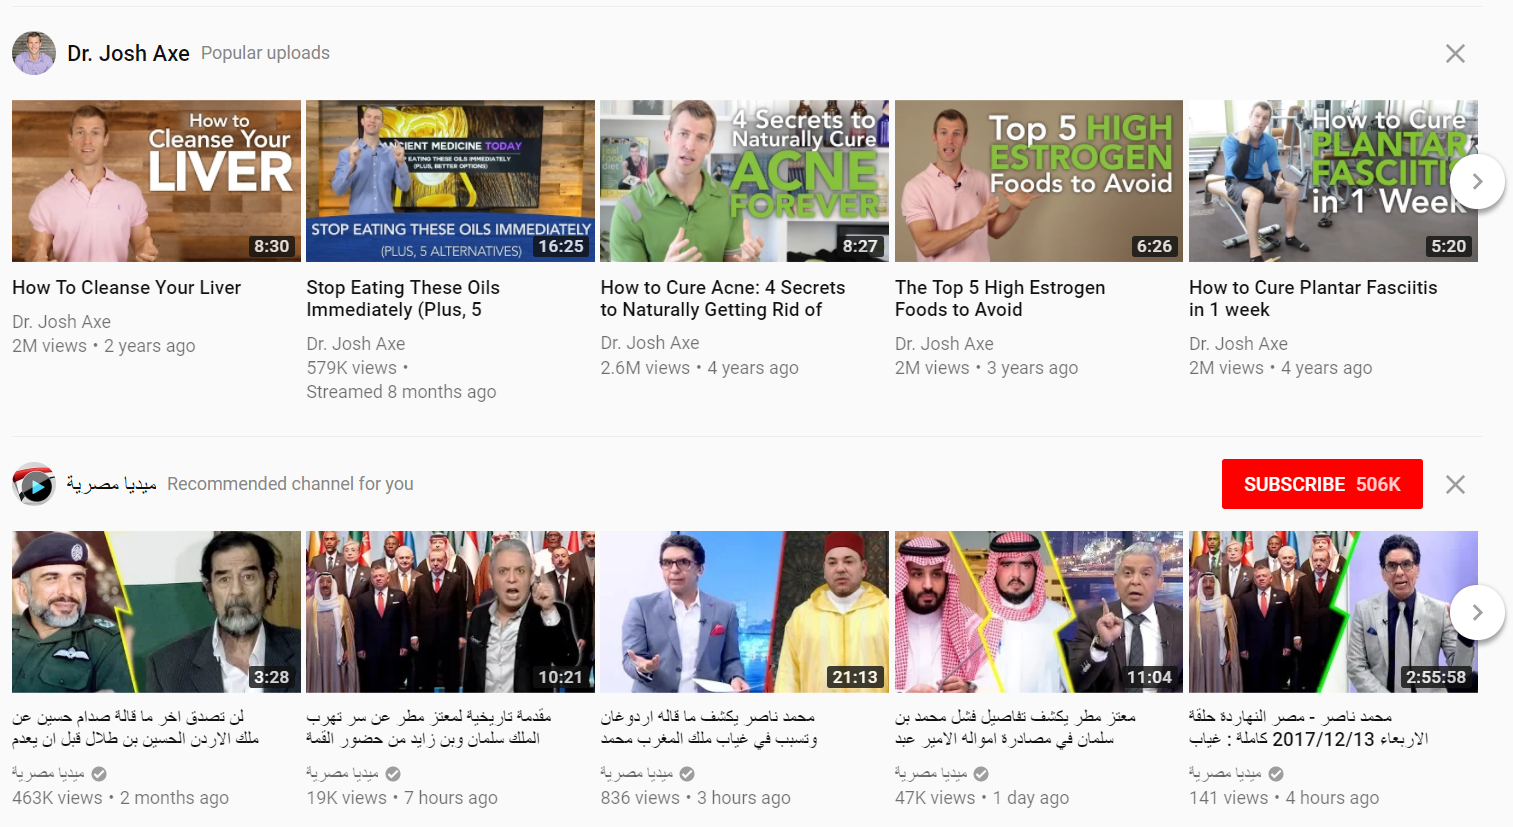
\includegraphics[scale=0.45]{Q3/yrc.png}
\end{figure}

\pagebreak

Youtube also shows a list of videos that I did not complete in case I wanted to continue to watch them. It also shows a list of recently uploaded videos that belong to categories in which I am interested based on my views history as the screen shot below shows.

\begin{figure}[h]
\caption{Recommended items by Youtube}
\centering
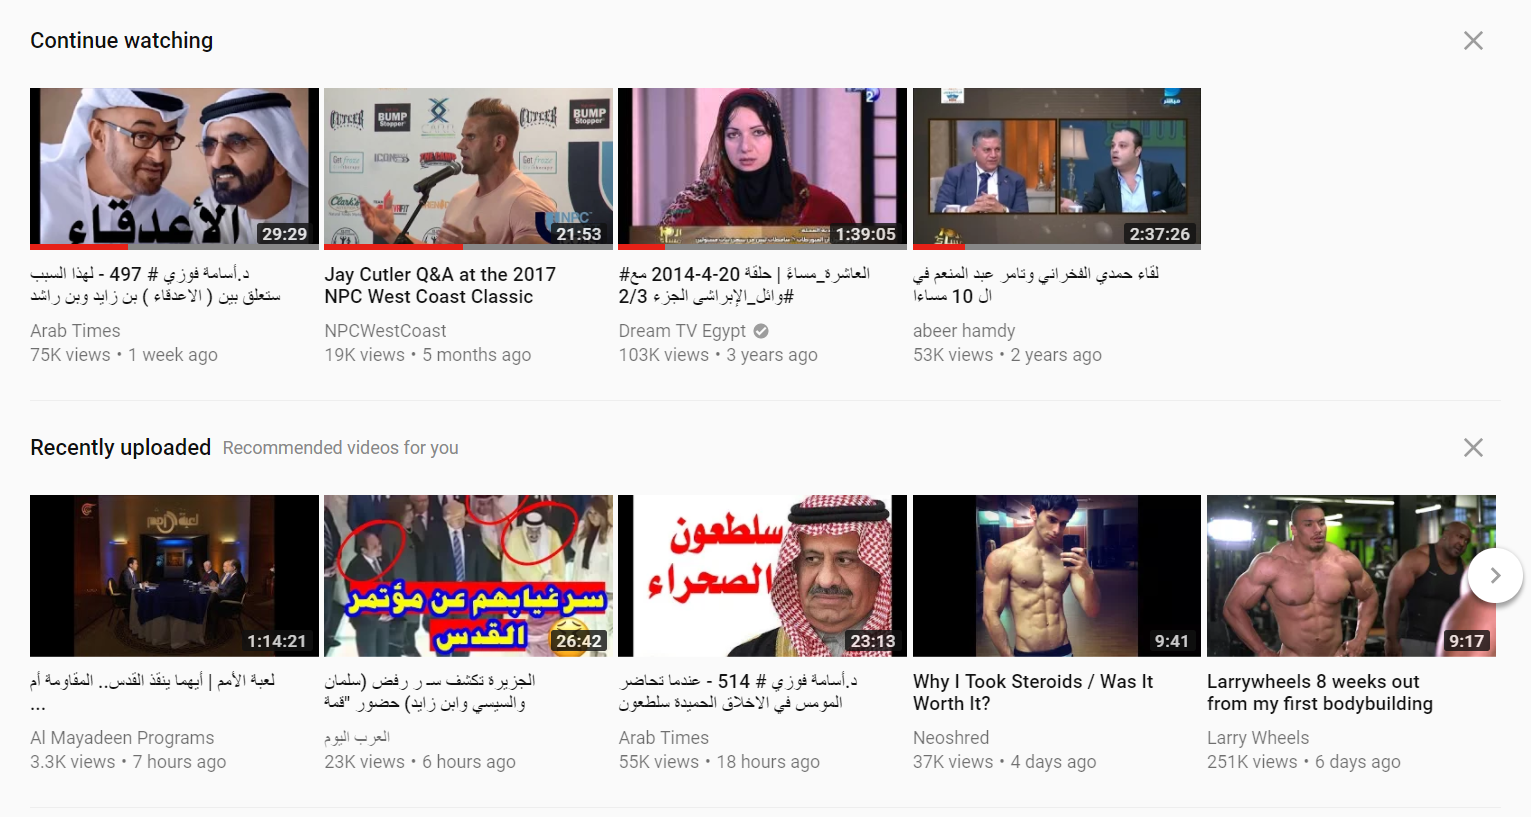
\includegraphics[scale=0.45]{Q3/yrr.png}
\end{figure}

\pagebreak

Youtube shows a list of live recommendations based on live channels I watch, mostly news. It also shows recommended a nonstop playlists ,Youtube mixes, based on a song or an atrist from my views history. I turned off recommended videos from one of the channels I am not interested in, RT Arabic. Youtube says: Got it. We'll tune your recommendations. It gave me the option to undo in case my cat turned that recommendation off for me. The screen shot below shows what I described.


\begin{figure}[h]
\caption{Recommended items by Youtube}
\centering
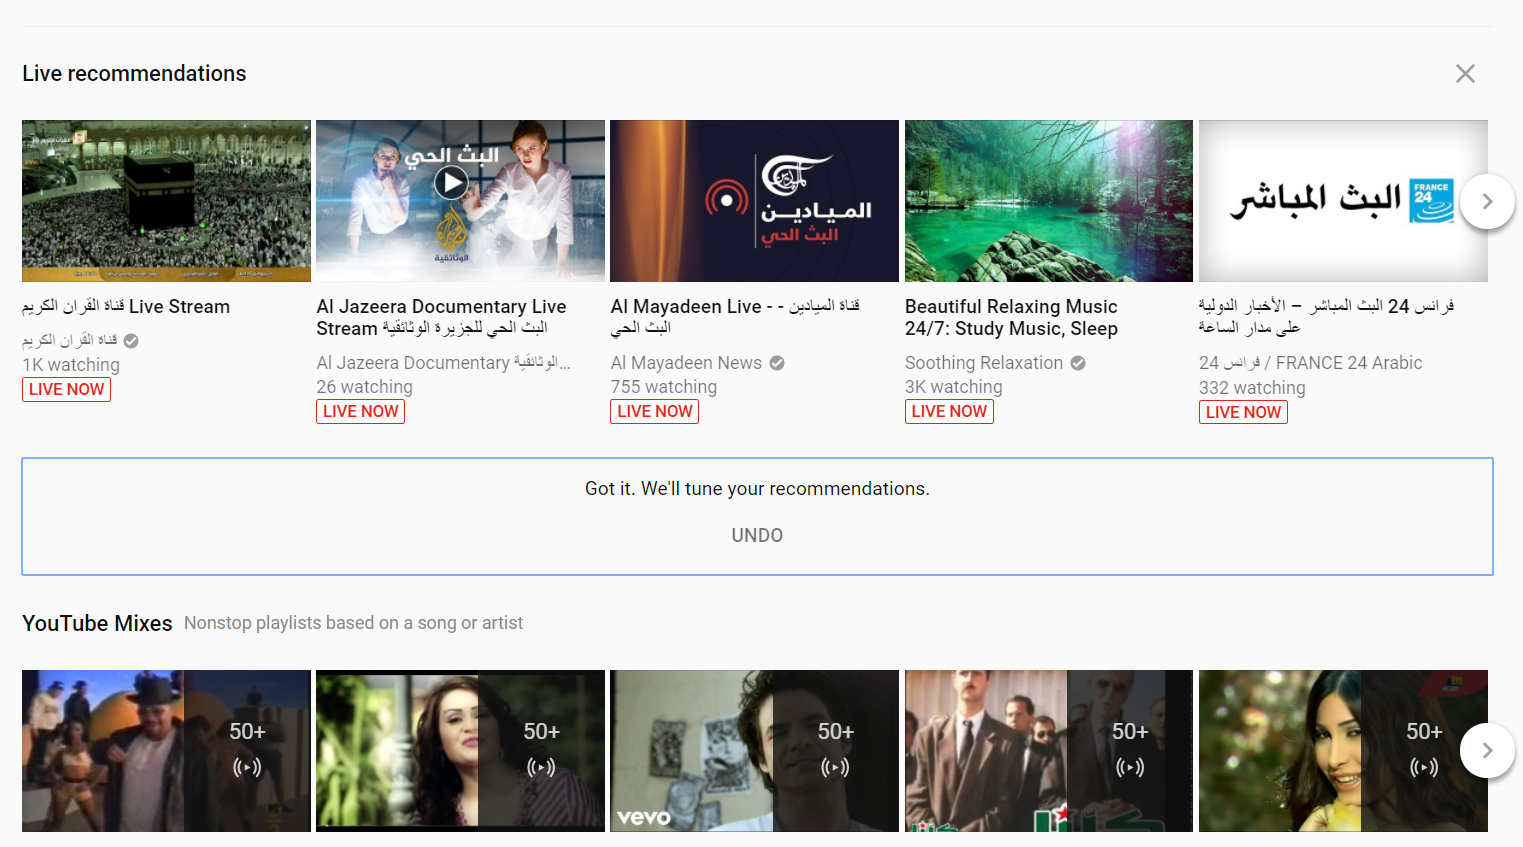
\includegraphics[scale=0.45]{Q3/yrp.png}
\end{figure}

\pagebreak

So far, it seems like Youtube is recommending the right videos for me, however, it also shows videos I am not interested in. This could be because these videos have so many views, millions, as seen in the next screen shot. I am not interested in Trailers, but Youtube shows it anyways.

\begin{figure}[h]
\caption{Recommended items by Youtube}
\centering
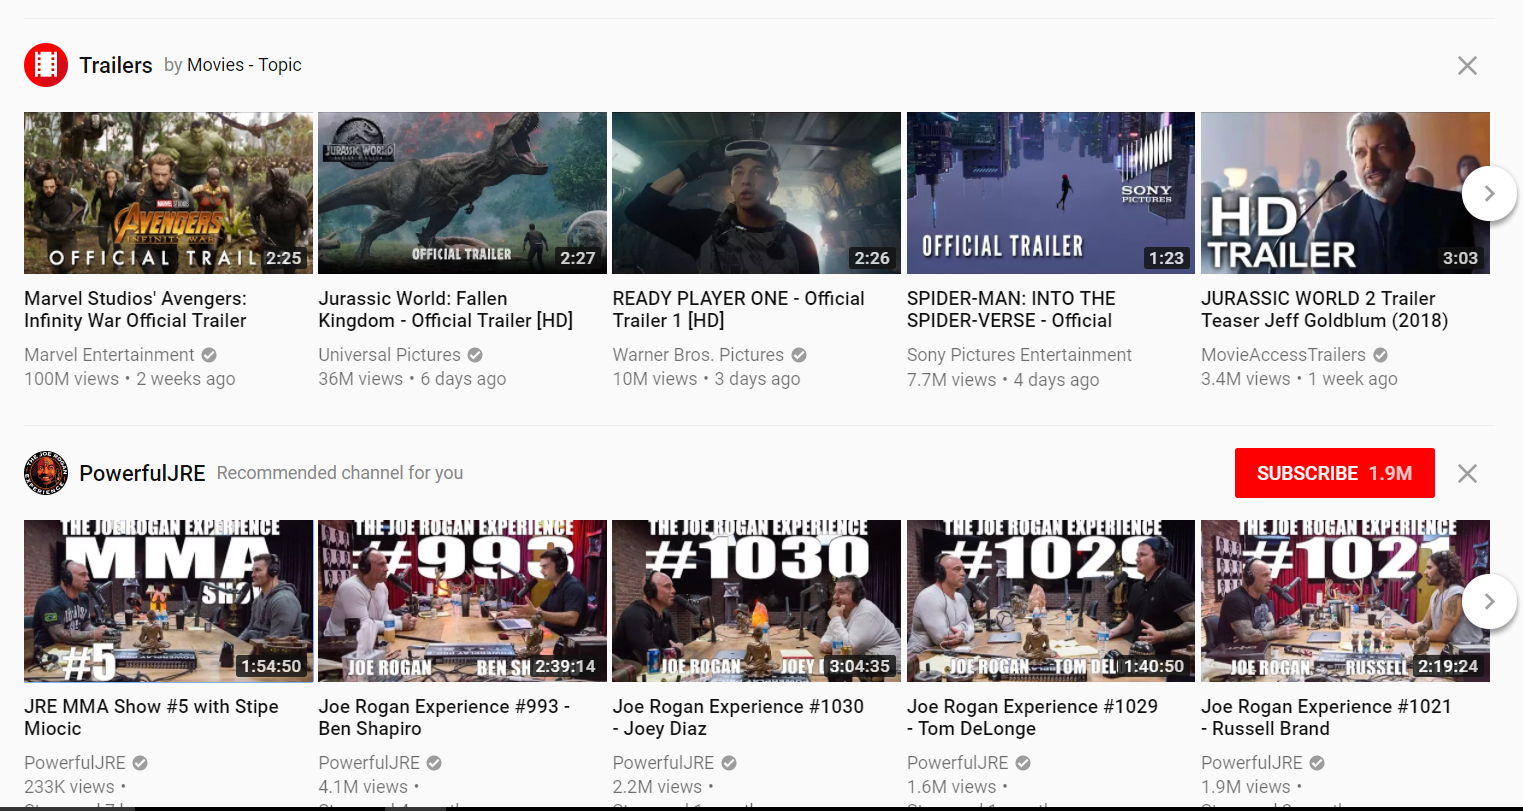
\includegraphics[scale=0.45]{Q3/yrt.png}
\end{figure}

\pagebreak

Finally, Youtube places an ad, sponsored video, in the upper right corner on  video pages I watch. The users who made these videos pay Youtube to show these videos to users based on the video that is on the same page. I have AdBlock installed on my browser so I do not have to see all kinds of advertisements. I disabled AdBlock to take the screen shot below.

\begin{figure}[h]
\caption{Recommended items by Youtube}
\centering
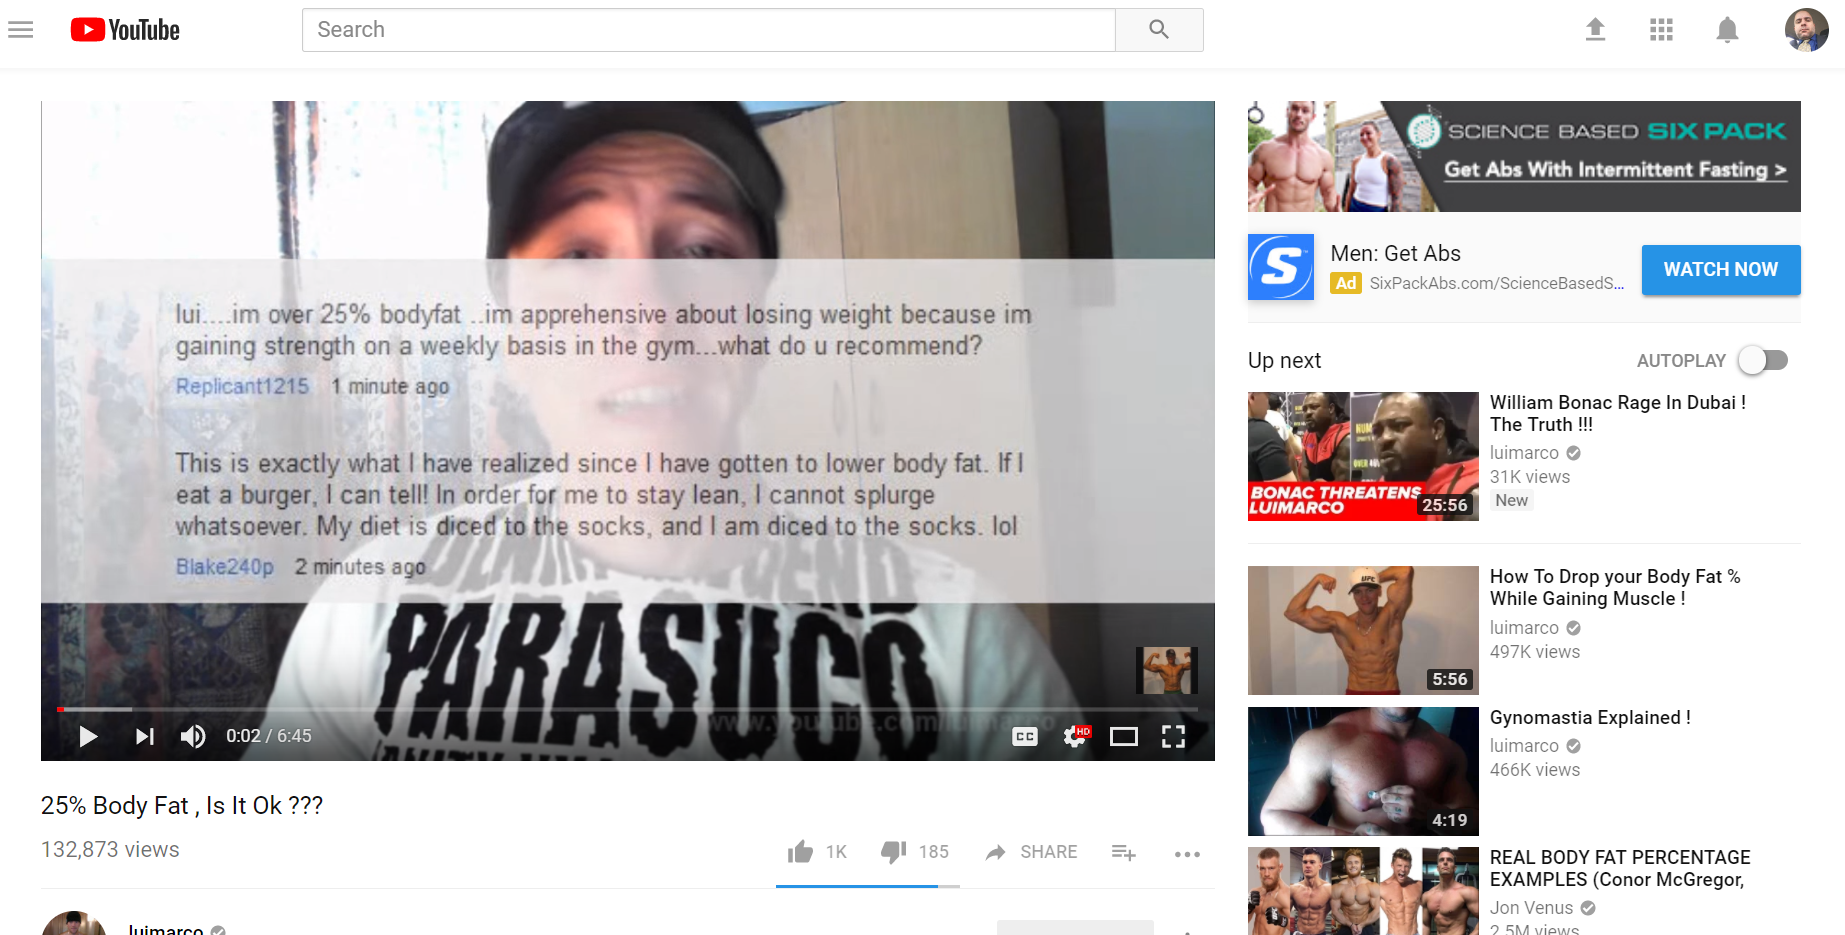
\includegraphics[scale=0.37]{Q3/yrs.png}
\end{figure}
 

 


\section*{Question 4:}
Exercise 7.2: 

Can you think of another measure of similarity that could be used in the vector space model? Compare your measure with the cosine correlation using some example documents and queries with made-up weights. Browse the IR literature on the Web and see whether your measure has been studied (start with van Rijsbergen’s book).


\subsection*{Answer:}

\section*{Question 5:}
Exercise 7.2: 

Can you think of another measure of similarity that could be used in the vector space model? Compare your measure with the cosine correlation using some example documents and queries with made-up weights. Browse the IR literature on the Web and see whether your measure has been studied (start with van Rijsbergen’s book).

\subsection*{Answer:}

In order for the similarity measure to give correct results when used in the vector space model, it must be based on the angle between the vectors. Any measure that is based on the Euclidean distance will give wrong results unless vectors, query \& documents' vectors, are reduced to the unit vectors, which is what cosine similarity does.

\textbf{Example:}

We have a query q = ``Do jealous people gossip?''. Let's assume that the two terms ``do'' and ``people'' are stop words. The two terms that affect the results are ``jealous'' and ``gossip''.

We also have three documents to examine, $d_1$, $d_2$, and $d_3$.

$d_1$: A document that is mostly about gossip, but has a little about jealousy.

$d_2$: A document about both gossip and jealousy. It has a little more about jealousy than it does about gossip. It is the most relevant document out of all three documents.

$d_3$: A document that is mostly about jealousy, but has a little about gossip.

Euclidean distance similarity will cause $d_1$ and $d_3$ to be ranked higher than $d_2$ with respect to the query q because the distance between q and $d_2$ is larger than the distance between q and $d_1$ as well as the distance between q and $d_3$. The result is clear in Figure 7 and Figure 8.

\begin{figure}[h]
\caption{Euclidean Distance Similarity Between Vectors}
\centering
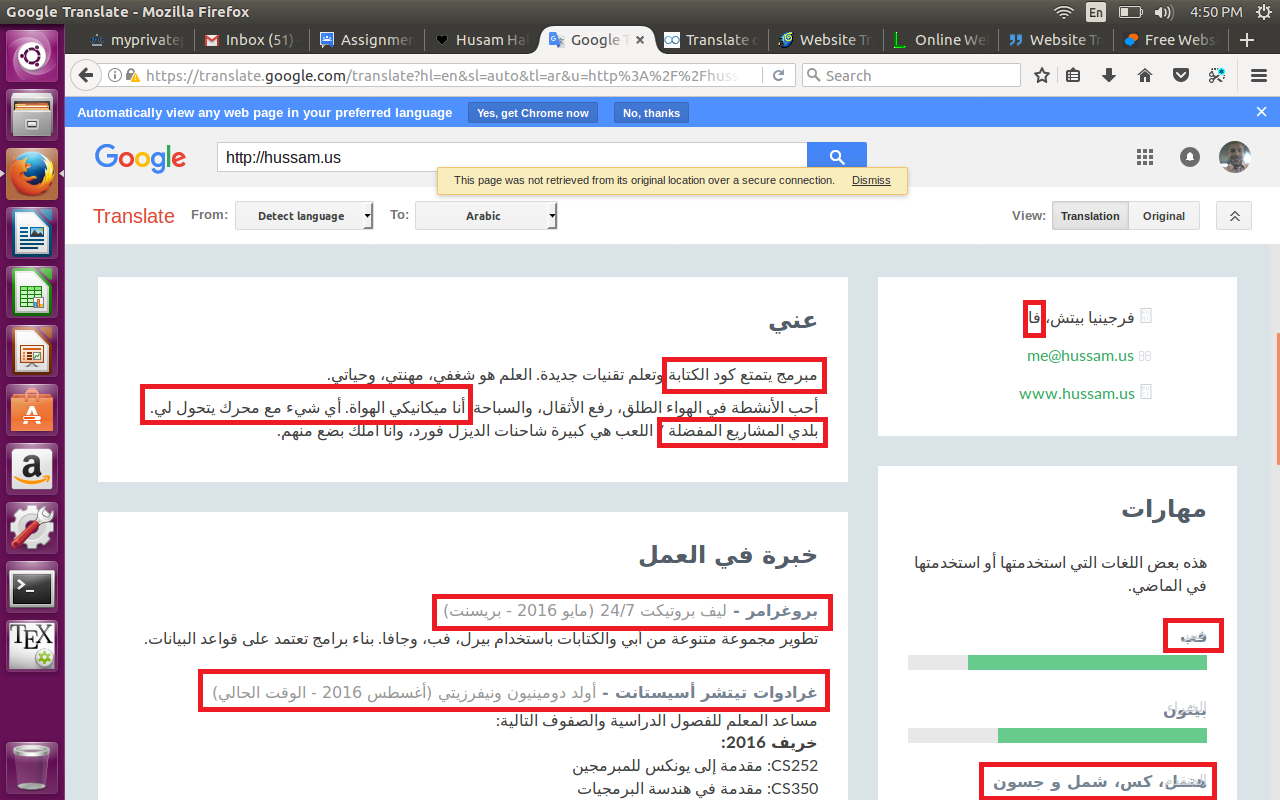
\includegraphics[scale=0.7]{Q5/1.png}
\end{figure}


\begin{figure}[h]
\caption{Euclidean Distance Similarity Between Vectors}
\centering
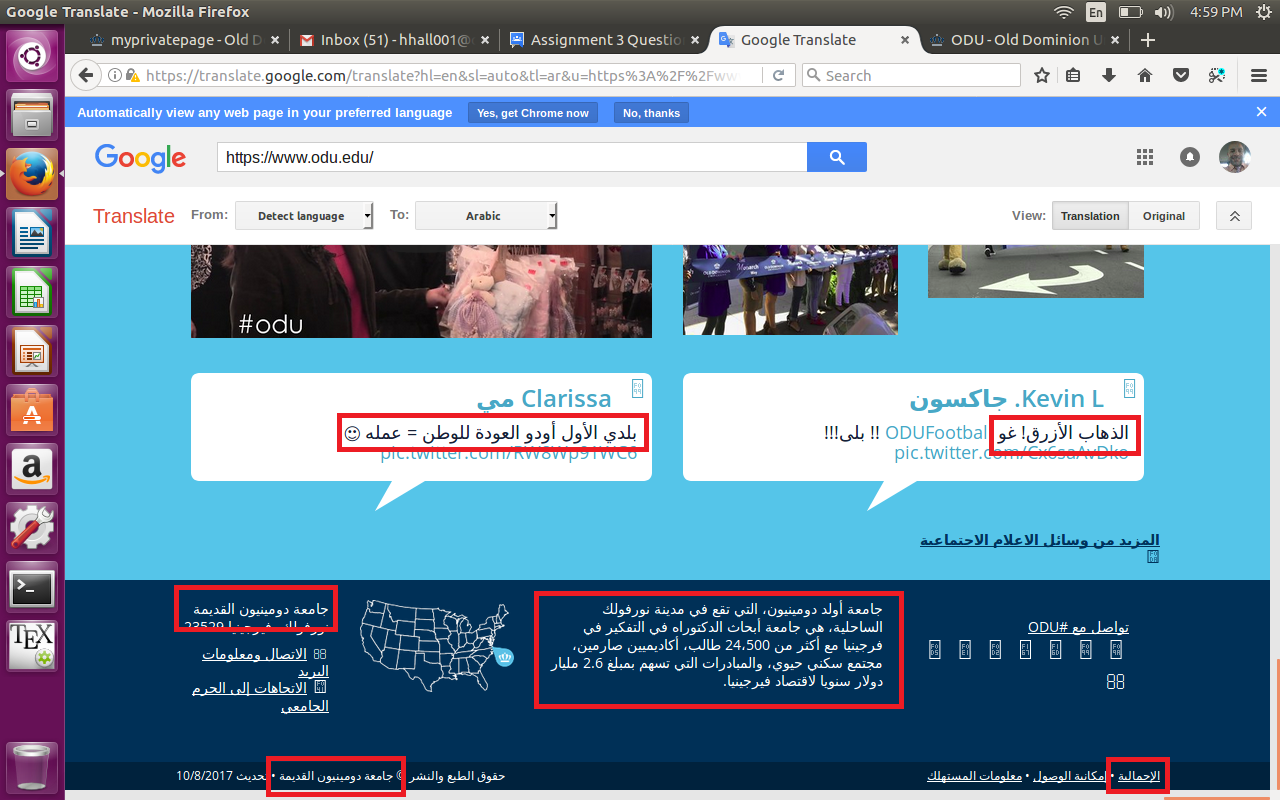
\includegraphics[scale=0.6]{Q5/2.png}
\end{figure}


The only case where Euclidean distance can be used as a similarity measure is when all vectors are reduced to the unit vector. This reduction can be performed by dividing each component in the vector by the vector's magnitude. The result is clear in Figure 9.

\begin{figure}[h]
\caption{Euclidean Distance Similarity Between Unit Vectors}
\centering
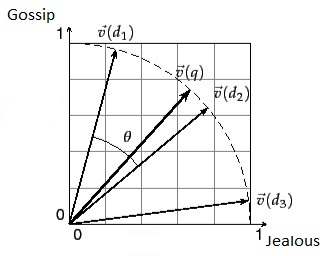
\includegraphics[scale=0.8]{Q5/4.jpg}
\end{figure}


\begin{figure}[h]
\caption{Cosine Similarity Between Vectors}
\centering
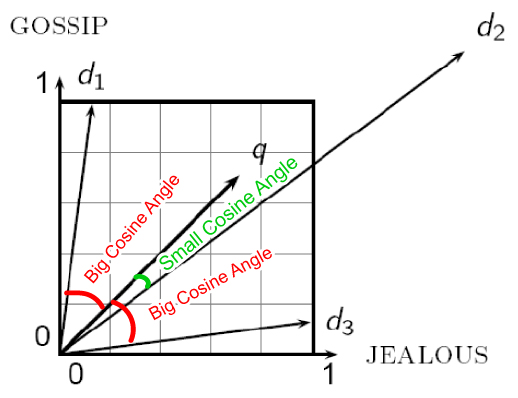
\includegraphics[scale=0.6]{Q5/3.jpg}
\end{figure}



The cotangent of the angle between vectors could be used as a measure of similarity in the vector space model. Cotangent $\theta$ is the reciprocal of tangent $\theta$. The graph of the function $y = cot(x)$ is shown in Figure 11.

\begin{figure}[h]
\caption{The graph of the function $y = cot(x)$}
\centering
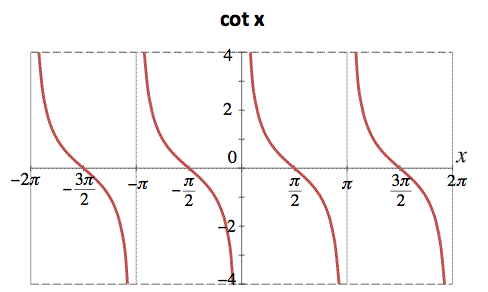
\includegraphics[scale=1.1]{Q5/graph_cot_pi.png}
\end{figure}


The period of the function cotangent that should be used lies in the interval $\theta = [0,\pi]$

From the graph, three statements can be made:

1. If the angle between the vectors is zero, the value of the cotangent is $\infty$.

2. If the angle between the vectors is $\frac{\pi}{2}$, the value of the cotangent is zero.

3. If the angle between the vectors is $\pi$, the value of the cotangent is $-\infty$.

This similarity measure agrees with the cosine similarity measure, but it is very steep since its value spans the interval $(-\infty,+\infty)$.

The log function can be wrapped around the cotangent function to reduce its aggression. 

$ similarity = \log_{10} (\cot(\theta))$

The base of the log is not important. Base 10 is not empirically determined. The base is there for completeness.

\textbf{Example with made-up weights:}

Let $q(8,9)$, $d_1(0,9)$, $d_2(25,25)$, and $d_1(9,0)$:

$$cos(q,d_1) = \frac{81}{108.374351209} = 0.747409319$$
$$\theta(q,d_1) = 41.63353931$$

$$cos(q,d_2) = \frac{425}{425.734659152} = 0.998274373$$
$$\theta(q,d_2) = 3.36646083$$

$$cos(q,d_3) = \frac{72}{108.374351209} = 0.664363839$$
$$\theta(q,d_3) = 48.36646065$$

$$log_{10}(cot(q,d_1)) = log_{10}(1.125) = 0.051152522$$

$$log_{10}(cot(q,d_2)) = log_{10}(17) = 1.230448921$$

$$log_{10}(cot(q,d_3)) = log_{10}(0.8889) = -0.051147094$$

\begin{longtable}{ |p{3cm}|p{3cm}|p{3cm}|p{3cm}| } 
\caption{Logarithmic Cotangent and Cosine Similarity Measures}\\    %%%%<===
\hline
Measure & $d_1$ & $d_2$ & $d_3$ \\
 \hline 
 Cosine & 0.747409319 & 0.998274373 & 0.664363839 \\
 \hline
  $log(cot)$ & 0.051152522 & 1.230448921 & -0.051147094 \\
 \hline
\end{longtable}

From the results, we can see that my measure agrees with the cosine correlation measure. The only noticeable difference is that the logarithmic cotangent correlation measure produced a negative value for the similarity between q and $d_3$. This negative result makes sense to a certain extent because $d_3$ is the document that is least related to q according to the results from the cosine similarity measure. My measure ranked the documents by their relevance to the query q as: $d_2, d_1, d_3$. The cosine correlation measure produced the same ranking.



 

\section*{Question 6:}
Exercise 7.7: 

What is the ``bucket'' analogy for a bigram language model? Give examples.

\subsection*{Answer:}

\section*{Question 7:}
Exercise 9.9: Use K-means and spherical K-means to cluster the data points in Exercise 9.8. How do the clusterings differ?

\subsection*{Answer:}

The data points from Exercise 9.8 are:
$$(-4,-2),(-3,-2),(-2,-2),(-1,-2),(1,-1),(1,1),(2,3),(3,2),(3,4),(4,3)$$


I wrote two simple python scripts to cluster the data points, ``k.py'' and ``sk.py'', using K-means and spherical K-means respectively.
I ran both programs for k = 2, 3, and 4.

The programs also generate plots for the data before and after clustering.

\subsection{K-means:}

\lstinputlisting[language=Python, breakatwhitespace=〈false), label=The content of k.py, caption= The content of k.py]{Q7/k.py}

\begin{lstlisting}[breakatwhitespace=〈false)]
hussam@hussam-HP-Compaq-nc8430-GE542UP-ABA:~/Desktop/99$ python k.py 2
hussam@hussam-HP-Compaq-nc8430-GE542UP-ABA:~/Desktop/99$ python k.py 3
hussam@hussam-HP-Compaq-nc8430-GE542UP-ABA:~/Desktop/99$ python k.py 4
\end{lstlisting}

\begin{figure}[h]
\caption{K-means for K = 1}
\centering
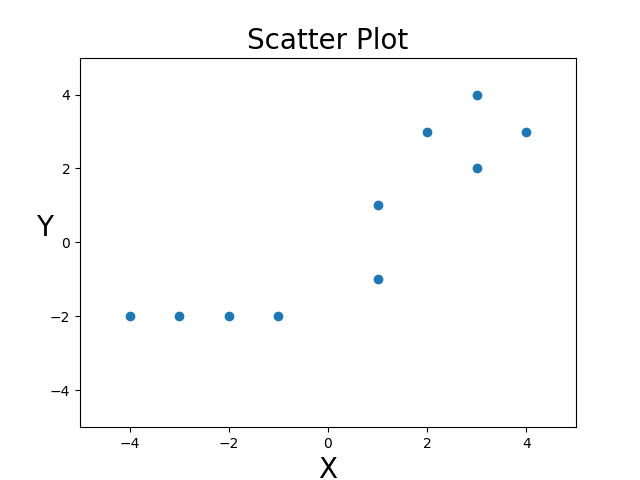
\includegraphics[scale=0.8]{Q7/k1.png}
\end{figure}

\pagebreak

\begin{figure}[h]
\caption{K-means for K = 2}
\centering
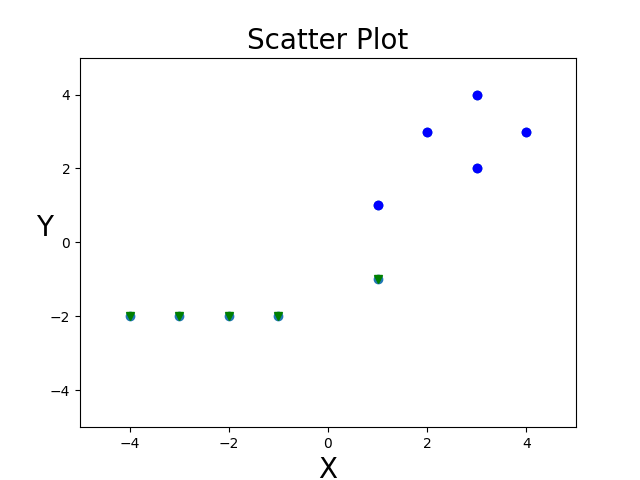
\includegraphics[scale=0.8]{Q7/k2.png}
\end{figure}

\pagebreak

\begin{figure}[h]
\caption{K-means for K = 3}
\centering
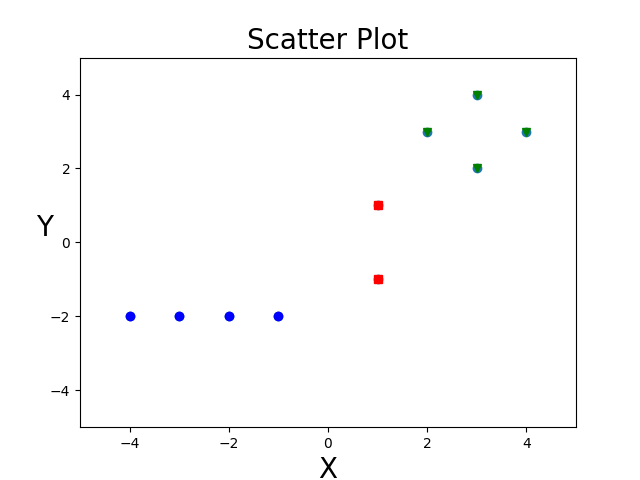
\includegraphics[scale=0.8]{Q7/k3.png}
\end{figure}

\pagebreak

\begin{figure}[h]
\caption{K-means for K = 4}
\centering
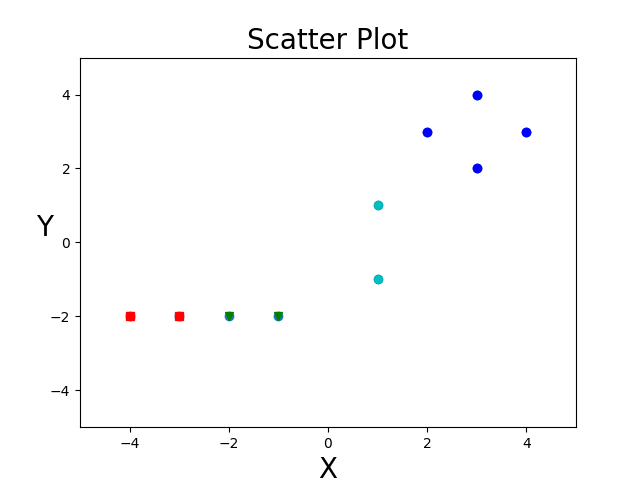
\includegraphics[scale=0.8]{Q7/k4.png}
\end{figure}

\pagebreak

\subsection{Spherical K-means:}

\lstinputlisting[language=Python, breakatwhitespace=〈false), label=The content of sk.py, caption= The content of sk.py]{Q8/sk.py}

\begin{lstlisting}[breakatwhitespace=〈false)]
hussam@hussam-HP-Compaq-nc8430-GE542UP-ABA:~/Desktop/99$ python sk.py 4
hussam@hussam-HP-Compaq-nc8430-GE542UP-ABA:~/Desktop/99$ python sk.py 3
hussam@hussam-HP-Compaq-nc8430-GE542UP-ABA:~/Desktop/99$ python sk.py 2
\end{lstlisting}

\pagebreak

\begin{figure}[h]
\caption{Spherical K-means for K = 2}
\centering
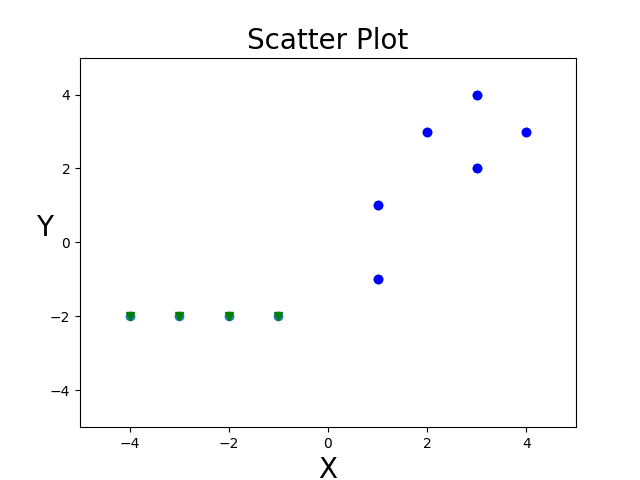
\includegraphics[scale=0.8]{Q7/sk2.png}
\end{figure}

\pagebreak

\begin{figure}[h]
\caption{Spherical K-means for K = 3}
\centering
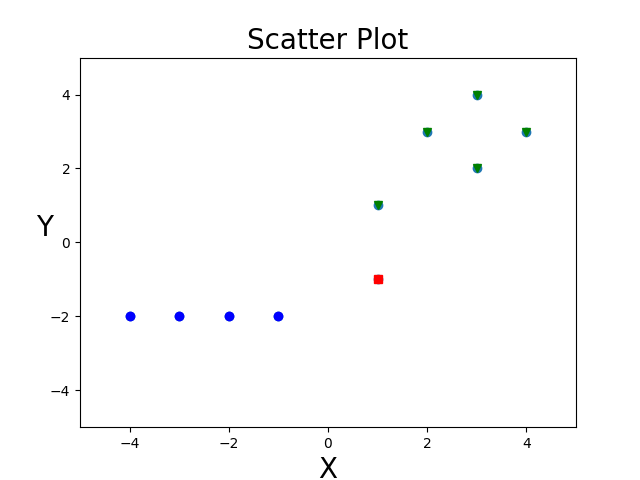
\includegraphics[scale=0.8]{Q7/sk3.png}
\end{figure}

\pagebreak

\begin{figure}[h]
\caption{Spherical K-means for K = 4}
\centering
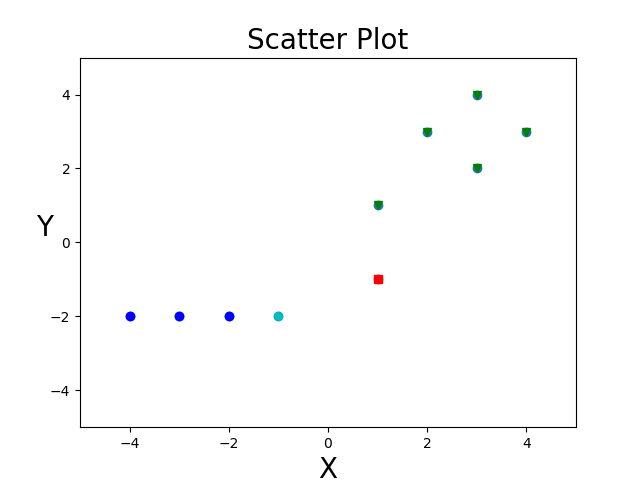
\includegraphics[scale=0.8]{Q7/sk4.png}
\end{figure}

\pagebreak


\textbf{Observation:}

K-means and Spherical K-means produced different results for all tested K values. The reason is that each clustering algorithm has a different approach to solve the clustering problem. K-means minimizes the Euclidean distance between the cluster center and the members of the cluster. The intuition behind this is that the radial distance from the cluster center to the element location should be similar for all elements of that cluster. On the other hand, Sperical K-means sets the center of the cluster such that it makes both uniform and minimal angle between components. The points should have consistent spacing between each other. That spacing is simpler to quantify as cosine similarity. 

\begin{thebibliography}{9}

\bibitem{} 
Stackoverflow. https://stackoverflow.com/questions/tagged/python.

\bibitem{}
http://convertjson.com/xml-to-json.htm

\bibitem{} 
https://docs.scipy.org/doc/scipy/reference/cluster.hierarchy.html

\bibitem{}
https://sourceforge.net/p/lemur/wiki/Galago\%20Query\%20Language/?version=2

\bibitem{}
https://matplotlib.org/api/\_as\_gen/matplotlib.pyplot.html\#module-matplotlib.pyplot


\end{thebibliography}


\end{document}